\documentclass{beamer}
\usepackage[utf8]{inputenc}

\usetheme{Madrid}
\usecolortheme{default}
\usepackage{amsmath,amssymb,amsfonts,amsthm}
\usepackage{txfonts}
\usepackage{tkz-euclide}
\usepackage{listings}
\usepackage{adjustbox}
\usepackage{array}
\usepackage{tabularx}
\usepackage{gvv}
\usepackage{lmodern}
\usepackage{circuitikz}
\usepackage{tikz}
\usepackage{graphicx}
\usepackage{multicol}
\setbeamertemplate{page number in head/foot}[totalframenumber]

\usepackage{tcolorbox}
\tcbuselibrary{minted,breakable,xparse,skins}



\definecolor{bg}{gray}{0.95}
\DeclareTCBListing{mintedbox}{O{}m!O{}}{%
  breakable=true,
  listing engine=minted,
  listing only,
  minted language=#2,
  minted style=default,
  minted options={%
    linenos,
    gobble=0,
    breaklines=true,
    breakafter=,,
    fontsize=\small,
    numbersep=8pt,
    #1},
  boxsep=0pt,
  left skip=0pt,
  right skip=0pt,
  left=25pt,
  right=0pt,
  top=3pt,
  bottom=3pt,
  arc=5pt,
  leftrule=0pt,
  rightrule=0pt,
  bottomrule=2pt,

  colback=bg,
  colframe=orange!70,
  enhanced,
  overlay={%
    \begin{tcbclipinterior}
    \fill[orange!20!white] (frame.south west) rectangle ([xshift=20pt]frame.north west);
    \end{tcbclipinterior}},
  #3,
}
\lstset{
    language=C,
    basicstyle=\ttfamily\small,
    keywordstyle=\color{blue},
    stringstyle=\color{orange},
    commentstyle=\color{green!60!black},
    numbers=left,
    numberstyle=\tiny\color{gray},
    breaklines=true,
    showstringspaces=false,
}
%------------------------------------------------------------
%This block of code defines the information to appear in the
%Title page
\title %optional
{12.130}
\date{October  2025}
%\subtitle{A short story}

\author % (optional)
{BEERAM MADHURI - EE25BTECH11012}



\begin{document}


\frame{\titlepage}
\begin{frame}{Question}
The linear operation $\mathrm{L}(\mathbf{x})$ is defined by the cross product $\mathrm{L}(\mathbf{x}) = \mathbf{b} \times \mathbf{x}$, where $\mathbf{b} = 
\begin{pmatrix}
0 \\
1 \\
0
\end{pmatrix}$ and $\mathbf{x} = \begin{pmatrix}
x_1 \\
x_2 \\
x_3
\end{pmatrix}$ are three dimensional vectors. The $3 \times 3$ matrix $\mathbf{M}$ of this operation satisfies $\mathrm{L}(\mathbf{x}) = \mathbf{M}\mathbf{x}$. Then the eigenvalues of $\mathbf{M}$ are

\begin{enumerate}[label=(\alph*)]
\begin{multicols}{2}
    \item $0, +1, -1$
    \item $1, -1, 1$
    \item $i, -i, 1$
    \item $i, -i, 0$
    \end{multicols}
\end{enumerate}
\end{frame}

\begin{frame}{Given Data}
    \begin{table}[h!]
    \centering
    \begin{tabular}[12pt]{ |c| c|}
    \hline
    \textbf{Point} & \textbf{Vector}\\ 
    \hline
    $\mathbf{v_1}$ &  $\myvec{1\\1\\1}$\\
    \hline
    $\mathbf{v_2}$ &   $\myvec{1\\-1\\1}$\\
    \hline
     $\mathbf{v_3}$ &  $\myvec{1\\1\\-1}$\\
    \hline
    \end{tabular}
    \caption{Variables used}
    \label{table 1.9.1}
\end{table}\\
\end{frame}
\begin{frame}{solution}
    \frametitle{finding the Normal:}
Given, \begin{align}L(x) = MX
\end{align}
\begin{align}L(x) = b \times X\end{align}

Cross product can be written as skew symmetric matrix.
\end{frame}
\begin{frame}
\begin{align}b \times X = \begin{pmatrix}0 & -b_3 & b_2 \\b_3 & 0 & -b_1 \\-b_2 & b_1 & 0\end{pmatrix}X\\
=\begin{pmatrix}0 & 0 & 1 \\0 & 0 & 0 \\-1 & 0 & 0\end{pmatrix}X\\
\therefore M =\begin{pmatrix}0 & 0 & 1 \\0 & 0 & 0 \\-1 & 0 & 0\end{pmatrix}\\
\end{align}
\end{frame}
\begin{frame}
finding eigenvalues :-

\begin{align}|M - \lambda I| = 0\end{align}
\begin{align}
\begin{pmatrix}-\lambda & 0 & 0 \\0 & -\lambda & 1 \\0 & -1 & -\lambda\end{pmatrix} = 0\\
-\lambda^3 - \lambda = 0\\
-\lambda(\lambda^2 + 1) = 0\\
\lambda_1 &= 0 \\\lambda_2 &= i \\\lambda_3 &= -i
\end{align}
Hence Option d is correct.
\end{frame}


\begin{frame}[fragile]
\frametitle{Python Code}
\begin{lstlisting}
import numpy as np
import matplotlib.pyplot as plt

# Define the matrix M
M = np.array([
    [0, 0, 1],
    [0, 0, 0],
    [-1, 0, 0]
])
\end{lstlisting}
\end{frame}

\begin{frame}[fragile]
\frametitle{Python Code}
\begin{lstlisting}
# Compute eigenvalues
eigenvalues = np.linalg.eigvals(M)
# Print eigenvalues
print("Eigenvalues of M:", eigenvalues)

# Plot eigenvalues in the complex plane
plt.figure(figsize=(6, 6))
plt.scatter(eigenvalues.real, eigenvalues.imag, color='red', s=100, label='Eigenvalues')
\end{lstlisting}
\end{frame}

\begin{frame}[fragile]
\frametitle{Python Code}
\begin{lstlisting}
plt.axhline(0, color='black', linewidth=0.5)
plt.axvline(0, color='black', linewidth=0.5)
plt.xlim(-1.5, 1.5)
plt.ylim(-1.5, 1.5)
plt.grid(True)
plt.title('Eigenvalues in the Complex Plane')
plt.xlabel('Real Part')
plt.ylabel('Imaginary Part')
plt.legend()
plt.show()
\end{lstlisting}
\end{frame}

\begin{frame}[fragile]
\frametitle{C Code}
\begin{lstlisting}
#include <stdio.h>
#include <math.h>
#include <complex.h>

int main() {
    // b = (0, 1, 0)
    // Cross product matrix M for b × x is:
    // |  0   0   1 |
    // |  0   0   0 |
    // | -1   0   0 |
\end{lstlisting}
\end{frame}

\begin{frame}[fragile]
\frametitle{C Code}
\begin{lstlisting}
    double M[3][3] = {
        {0, 0, 1},
        {0, 0, 0},
        {-1, 0, 0}
    };

    // Characteristic equation of M:
    // |M - λI| = 0 gives  λ(λ^2 + 1) = 0
    // ⇒ λ = 0, i, -i
\end{lstlisting}
\end{frame}

\begin{frame}[fragile]
\frametitle{C Code}
\begin{lstlisting}
    double complex eigen1 = 0.0 + 0.0 * I;
    double complex eigen2 = 0.0 + 1.0 * I;
    double complex eigen3 = 0.0 - 1.0 * I;
    printf("The eigenvalues of matrix M are:\n");
    printf("λ1 = %.1f + %.1fi\n", creal(eigen1), cimag(eigen1));
    printf("λ2 = %.1f + %.1fi\n", creal(eigen2), cimag(eigen2));
    printf("λ3 = %.1f + %.1fi\n", creal(eigen3), cimag(eigen3));
    return 0;
}
\end{lstlisting}
\end{frame}

\begin{frame}[fragile]
\frametitle{Python and C Code}
\begin{lstlisting}
import numpy as np

def calculate_eigenvalues():
    # b = (0, 1, 0)
    # Cross product matrix M for b × x is:
    # |  0   0   1 |
    # |  0   0   0 |
    # | -1   0   0 |
\end{lstlisting}
\end{frame}

\begin{frame}[fragile]
\frametitle{Python and C Code}
\begin{lstlisting}
    # Define the 3x3 matrix M using a NumPy array
    M = np.array([
        [0, 0, 1],
        [0, 0, 0],
        [-1, 0, 0]
    ])
    # Calculate the eigenvalues and (optionally) eigenvectors
    # 'w' will contain the eigenvalues (complex numbers)
    w, v = np.linalg.eig(M)
    # Note: The characteristic equation λ(λ^2 + 1) = 0 yields 
    # λ = 0, i, -i. The calculated values should match these.
\end{lstlisting}
\end{frame}

\begin{frame}[fragile]
\frametitle{Python and C Code}
\begin{lstlisting}    
    # Sort the eigenvalues for consistent output order (optional)
    # Sorting a mix of real and complex numbers can be tricky; 
    # we'll just print them as they come out for simplicity, 
    # which is usually (0+0j), (0+1j), (0-1j) or a permutation.

    print("The eigenvalues of matrix M are:")
    # Use a loop to print each eigenvalue
    for i, eigenvalue in enumerate(w):
\end{lstlisting}
\end{frame}

\begin{frame}[fragile]
\frametitle{Python and C Code}
\begin{lstlisting}
        # NumPy returns eigenvalues as complex numbers (even if the imaginary part is zero)
        # We can format the output to match the C code style (real + imag*i)
        print(f"λ{i+1} = {eigenvalue.real:.1f} + {eigenvalue.imag:.1f}i")
# Execute the function
if __name__ == "__main__":
    calculate_eigenvalues()
\end{lstlisting}
\end{frame}

\begin{frame}
\begin{figure}[H]
    \centering
    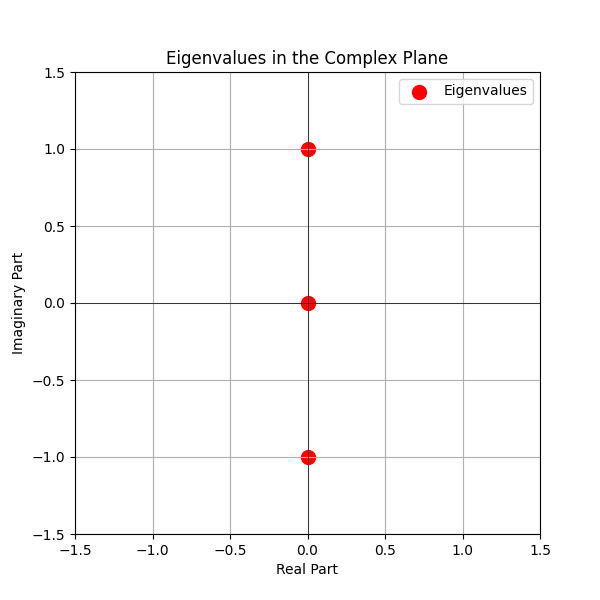
\includegraphics[width=0.75\columnwidth]{graph-20.png}
    \caption{Plot}
    \label{fig:placeholder}
\end{figure}
\end{frame}

\end{document}